\section{Economic authorization before certification}
\label{sec:economic-authorization}
Requiring evidence before any exposure is an investment constraint as well as
an inferential choice. A manager can instead authorize a provisional position
using training estimates, while keeping a separate OOS evidence process.
This accepts economic risk before certification. It does not strengthen the
statistical guarantee. We study that distinction in a controlled companion
experiment, retaining the complete adaptive-fund comparison separately.

\subsection{The comparison certified by an increase in exposure}
An improvement of a full target over cash does not imply that increasing an
existing provisional position is beneficial. For a fixed target $w$, write
$m_1=\E[w'A_{t+1}\mid\F_t]$ and
$m_2=\E[(w'A_{t+1})^2\mid\F_t]$. Starting from $qw$, with $0<q<1$ and
$\Lambda_t=I$, the one-period gain from increasing to $w$ rather than
retaining $qw$ is
\begin{align}
 J_t(w;qw)-J_t(qw;qw)
 ={}&(1-q)m_1-\frac{\gamma}{2}(1-q^2)m_2\notag\\
 &-c(1-q)\|w\|_1-\frac{\eta}{2}(1-q)^2\|w\|_2^2.
 \label{eq:authorization-increase}
\end{align}
This differs from $J_t(w;0)-J_t(0;0)$. With no costs, $\gamma=1$,
$m_1=.6$, $m_2=1$ and $q=.5$, full exposure has expected utility $.1$,
whereas half exposure has $.175$. A positive cash-entry gain therefore
coexists with a negative gain from increasing exposure.
If an increase is to be statistically certified, its own candidate/reference
score needs a valid evidence process and appropriate error allocation.
Retaining the original cash comparison retains its original interpretation.

\subsection{A common candidate and a training-based economic gate}
The existing Greedy fund fits weights from training but ranks moves by an
accumulated OOS score mean. It is not a training-only investment authorization
rule. The new experiment selects one candidate using only the initial training
year and then keeps its identity fixed. All four methods share its annually
updated target, the fitting calendar and observed returns.

Let $\widehat\mu_j$ be its training mean, $\widehat M_{jj}$ its sample raw
second moment plus the fixed ridge, and $\widehat s_j$ its mean's working HAC
standard error. The latter uses Bartlett weights and bandwidth
$\min(20,n-1)$. With $H=252$ and $z=1.6448536$, the scalar target is
\[
 \widehat w_j=\operatorname{clip}_{[-L,L]}
 \left\{\frac{\operatorname{sign}(\widehat\mu_j)
  (|\widehat\mu_j|-z\widehat s_j-c/H)_+}
  {\gamma\widehat M_{jj}+\eta/H}\right\}.
\]
Initially the candidate maximizes
\[
 \widehat V_j(w;0)
 =H\{w\widehat\mu_j-z|w|\widehat s_j
                 -\gamma w^2\widehat M_{jj}/2\}-C(w,0).
\]
Subsequent fits use the expanding observed history of that same candidate.
The standard-error penalty is a working economic adjustment, not a
finite-sample or post-selection confidence guarantee. The holding forecast
amortizes entry costs over $H$ dates; actual funds charge costs when incurred.

Economic quarter takes $q\widehat w_j$, $q=.25$, when its penalized forecast
is positive. Economic full takes $\widehat w_j$ when its corresponding
forecast is positive. Neither requires statistical evidence.
Wait holds cash before a shared full-exposure authorization; Hybrid holds
the provisional position before that date. Afterwards both target
$\widehat w_j$. At an annual review, authorization requires shadow log
evidence at least $\log20$, a historical score mean above the unchanged
$10^{-8}$ floor, and positive current training forecasts for full exposure
and the increase. Forecast gates require more than $H\times10^{-8}$,
matching the daily utility floor. The shared increase forecast is evaluated from the
provisional fund's previous allocation. It uses the $H$-date holding
criterion rather than the one-period quantity in
\eqref{eq:authorization-increase}. Decisions first trade on the next date.

The shared corrected-tail process compares a full shadow policy with cash;
its public certificates and nine betting components are unchanged. Predictable
provisional investment does not feed that shadow process through fund wealth
or trading state. This construction preserves an individual conditional-null
comparison; it does not certify the actual exposure increase or current
profitability. Each actual fund pays its own costs and retains absorbing
insolvency. The complete horizon includes noncrossings and losses.

\subsection{Executed comparison and its interpretation}
The numerical rules were committed before generating the new seeds
70001--70100, after the earlier pilot and the economic-authorization discussion.
They were not registered before those earlier observations. All 100 new
markets use the same 500-stock, 100-signal financial DGP, one training year
and 14 OOS years. They are not pooled with the separate adaptive-fund study.
Independent arithmetic replay covers every new market; two fixed seed
identifiers additionally receive complete independent market and public
moment-certificate replays.

\begin{table}[H]\centering\small
\begin{tabular}{lrrrr}\toprule
Method & Net utility & MC SE & Mean wealth & Mean max DD\\\midrule
Wait & 0.003655 & 0.000581 & 1.057 & 0.25\% \\
Economic quarter & 0.010747 & 0.000412 & 1.165 & 0.47\% \\
Hybrid & 0.013482 & 0.000805 & 1.217 & 0.63\% \\
Economic full & 0.042602 & 0.001652 & 1.875 & 1.88\% \\
\bottomrule\end{tabular}
\caption{Controlled exposure timing on all 100 fresh markets. Utility is mean
daily realized quadratic utility net of actual costs, multiplied by 252;
it is not annual return or certainty equivalent. Wealth starts at one and
compounds over 14 OOS years. DD denotes each path's maximum drawdown,
averaged across markets. All four methods retain noncrossings and losses.}
\label{tab:economic-authorization}
\end{table}
The primary paired Hybrid-minus-Wait utility difference is $0.009828$, with approximate pointwise 95\% Monte Carlo interval $[0.009219,0.010436]$. Hybrid-minus-Economic-full is $-0.029119$ with interval $[-0.030956,-0.027283]$; this secondary contrast is unadjusted. Evidence crosses at an annual review in 38 markets. 35 full-exposure authorizations are executed; 3 first crossings occur only at the terminal review. Intervals use the 100 paired markets and Student $t_{99}$, not daily observations.

All 100 markets initiate provisional exposure. In 0 markets the provisional period has negative cumulative realized utility, but the evaluator records 784 pre-deployment dates with negative conditional utility. These descriptive observations do not certify an absence of downside risk. All 1,400 annual target fits bind at the leverage cap; 0 markets change their target. Consequently the experiment identifies exposure timing for selected positions, without validating the uncertainty calibration or adaptive target sizing.

\begin{figure}[H]\centering
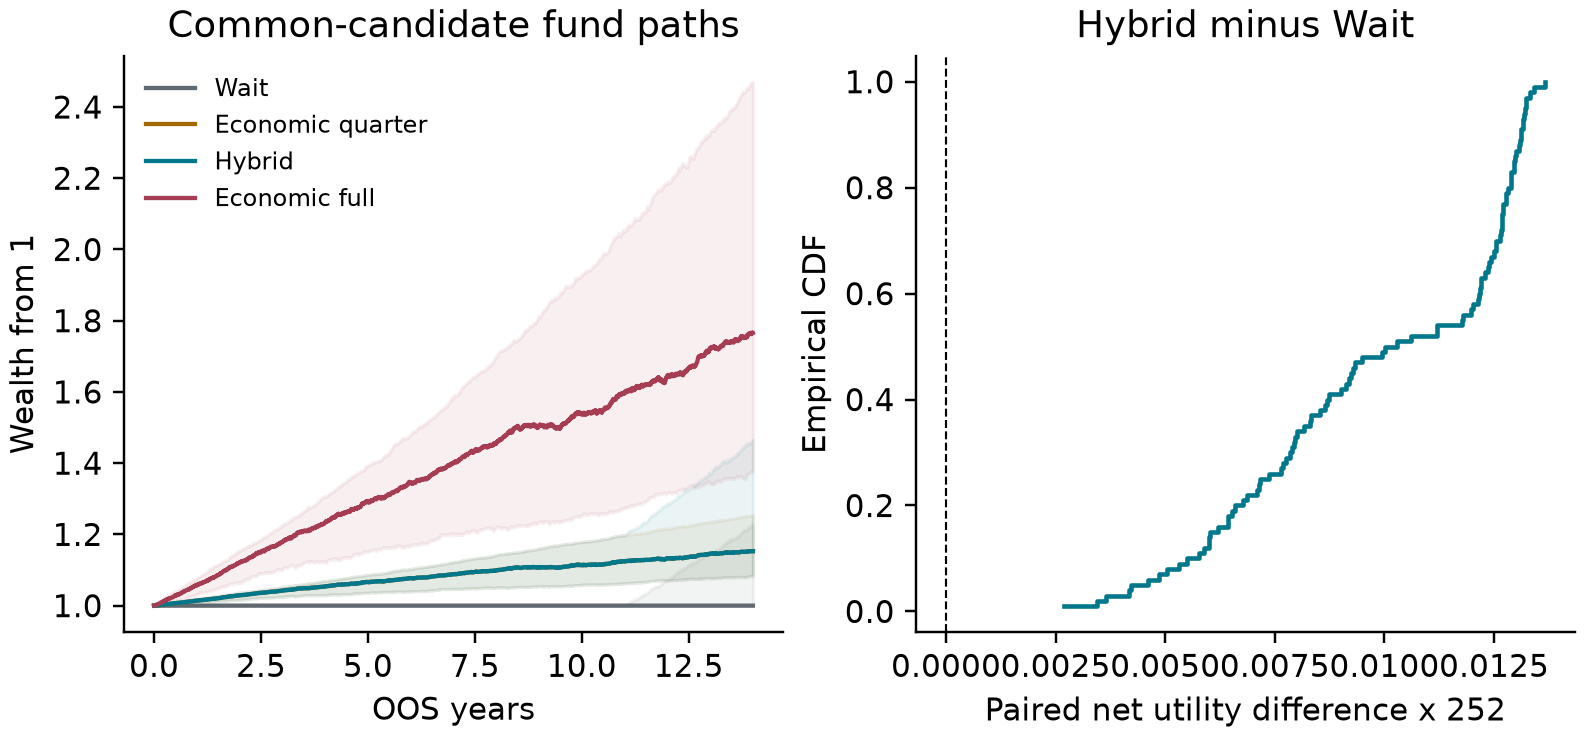
\includegraphics[width=\linewidth]{figures/economic_authorization.png}
\caption{All 100 new markets. Left: median wealth with 10th--90th market
quantiles, not confidence bands. Right: paired Hybrid-minus-Wait utility
differences. The candidate and fitting schedule are common; each fund pays
its own actual costs.}
\label{fig:economic-authorization}
\end{figure}
\FloatBarrier


For actual fractions $\theta_t^P,\theta_t^W$ and a common full-target return
$X_t=w_t'A_t$, the realized paired utility difference is exactly
\[
 \sum_t\left[(\theta_t^P-\theta_t^W)X_t
 -\frac{\gamma}{2}\{(\theta_t^P)^2-(\theta_t^W)^2\}X_t^2
 -(C_t^P-C_t^W)\right].
\]
Before insolvency the common post-authorization targets cancel the return
and quadratic-risk terms; transition costs remain different. If insolvency
stops one fund, use its actual zero exposure in this general identity.
The companion therefore isolates provisional exposure for a specified common
candidate and evidence clock. It does not attribute the complete adaptive
funds' performance gap solely to waiting. Under this DGP, provisional exposure
recovers utility relative to waiting; immediate full exposure has greater
utility and greater average drawdown than Hybrid. That tradeoff supplies
economic evidence without making certification a profitability guarantee.
